% \Huge

\section{Cosmological Context}

Cosmology has seen many important advances in the last few decades. Piece by piece we are uncovering the history of the universe and it's components. We now know that our galaxy is just one in trillions (\cite{2016ApJ...830...83C}), and part of a rapidly expanding universe.

Our two main observational tools today are the Cosmic Microwave Background (CMB) and Galaxy Surveys. From the CMB we learn about the primordial universe, and Galaxy Surveys uncover the nature and structure of the Universe at late times. The latest surveys like Planck (\cite{2016A&A...594A..13P}), SDSS \todo{ref} or DES \todo{ref} lend strong support to the $\Lambda CDM$ paradigm. Within this Cosmological Standard Model we now understand most of the important events that shaped the history of our Universe and dictate its future. 

The two most important components of this model are arguably Dark Matter and Dark Energy. The two account for a total of about $95\%$ of the matter-energy budget of the universe (e.g. \cite{2016A&A...594A..13P}). We have been able to constrain the properties of the two mysterious components quite well. Most observational probes are consistent with a Cosmological Constant model of dark energy \todo{ref}, but they don't yet exclude other models like quintessence \todo{ref}. On the other hand, the Cold Dark Matter model of a non-interacting (or very weakly interacting) particle that only has gravitational impact is leading on the dark matter side \todo{ref}. However, despite this wealth of knowledge, the nature of the two most important components of the Universe still eludes us.

The most important gaps in our knowledge of this Cosmological history are either related to the very early universe (long before the CMB was emitted) or to the evolution of the Universe between recombination and the first galaxies being formed. In this project we will investigate this second gap in an effort to bring some light on an era that is referred to as the Dark Ages. \todo{this is not necessarily our main focus though}

\section{The Cosmic Microwave Background}

The Cosmic Microwave Background is our main observational tool for studying the early universe. It is the first light emitted in the Universe after recombination, and it encodes plenty of useful information. The CMB is the most perfect black body ever observed (\cite{1999dpf..conf.....W}). Its existence is already a strong proof in support of the Big Bang model. On the other hand, the anisotropies found in the CMB strongly support both the $\Lambda CDM$ paradigm and Inflation.

CMB surveys have measured these anisotropies very accurately (Figure~\ref{fig:1.1}). They are key in understanding the matter distribution in the universe. Before recombination Baryons and Radiation were coupled, so the matter distribution at recombination was imprinted in the CMB distribution. The matter distribution then continued to evolve on its own into the large scale structure we see today. Among the key anisotropies detected in the CMB are Baryon Acoustic Oscillations. This feature is a result of oscillations in the primordial Baryon-Photon plasma. Radiation opposed the collapse of baryonic matter into the potential wells created by collapsing dark matter (which does not interact and is free to collapse). This produced acoustic waves that were imprinted in both the matter distribution (we detect it today in the galaxy distribution) and the radiation distribution (we detect it in the CMB). This probe lends strong support both to the existence of dark matter which plays a key role in their creation, and to that of dark energy (as a cosmological constant) which dictates their evolution at late times.

\begin{figure}
    \centering
    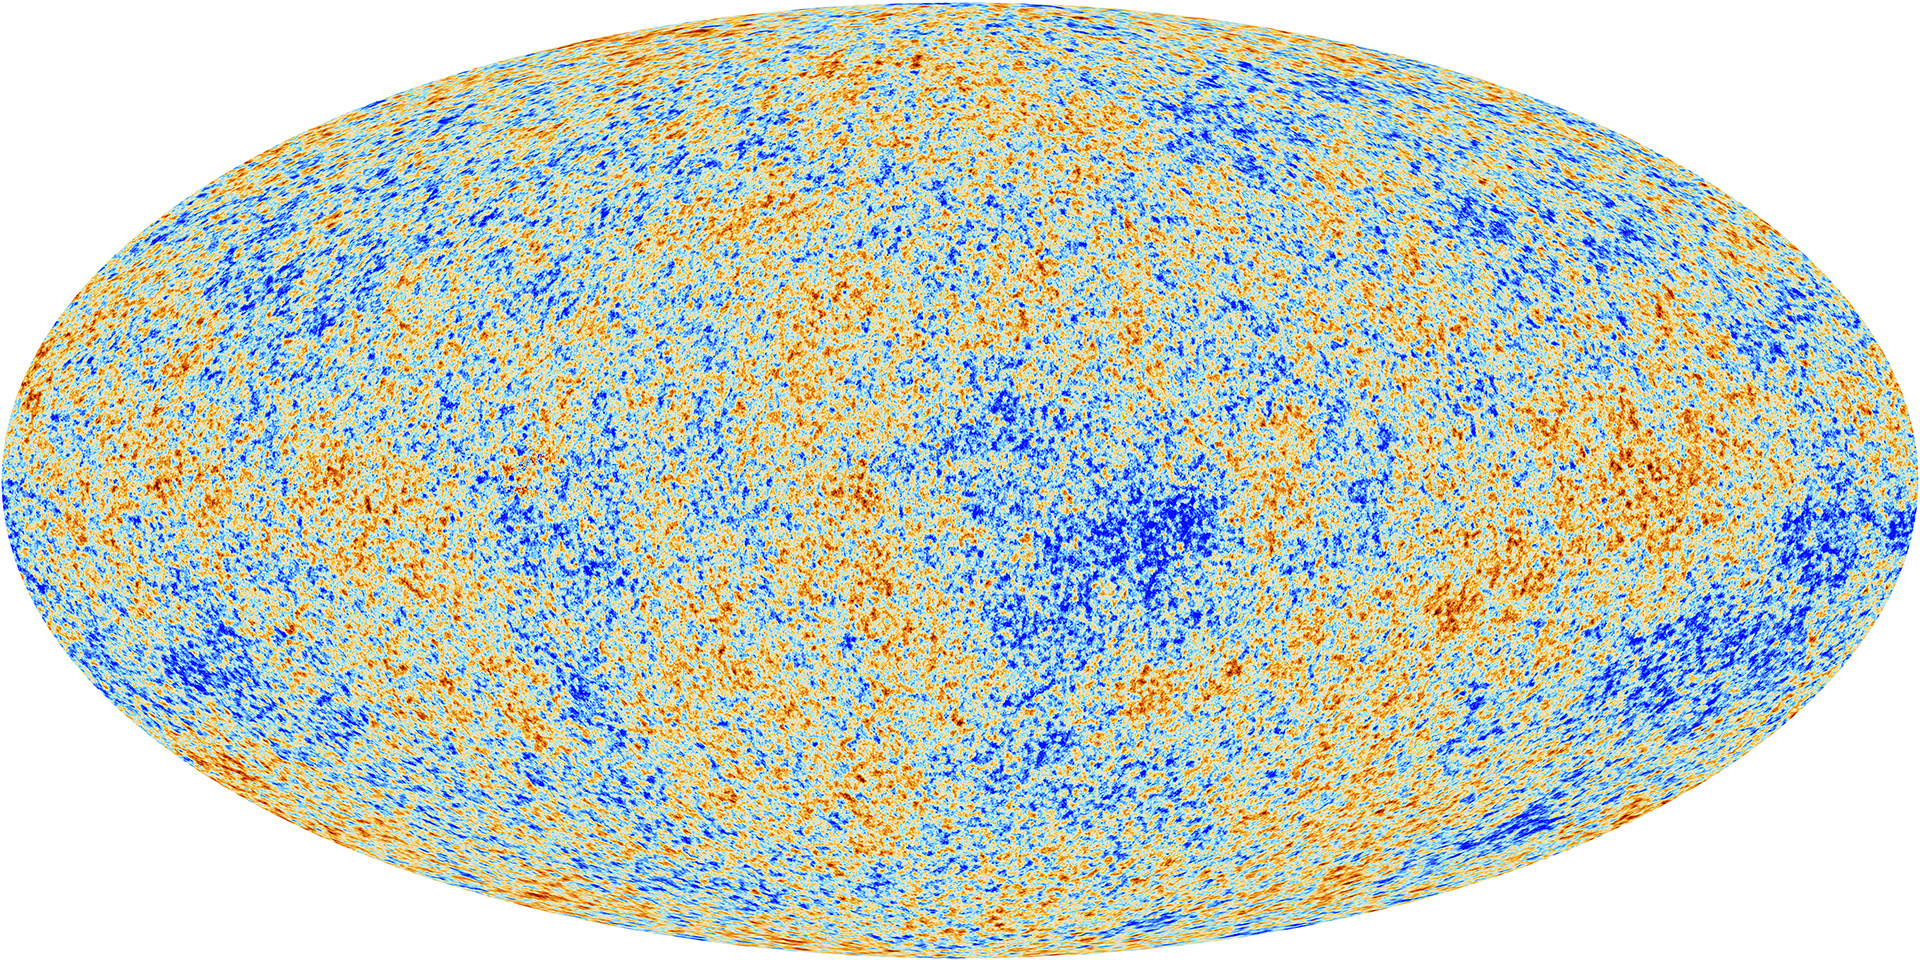
\includegraphics[width=0.9\columnwidth]{images/misc/Planck_CMB.jpg}%
    

    \caption{
    Map of the Cosmic Microwave Background acquired by the Planck Space Telescope (\cite{2016A&A...594A..13P}). After subtracting the effect of our own motion relative to the CMB, the anisotropies only start appearing at $10^{-5} K$. This gives us a glimpse into the primordial matter distribution.
    }
    
    \label{fig:1.1}
\end{figure}

The CMB also has plenty of data in support of Inflation. It shows a uniform, very flat universe that contains mostly gaussian anisotropies. All of these are outcomes of inflation and are hard to explain without it. Of particular interest for us are the gaussian anisotropies. There are many models of inflation \todo{refs!!}, and at the moment we do not have enough precision to distinguish between them. Most models predict some primordial non-gaussianity, however constraining this is key to differentiating between them \todo{ref}.

After the CMB was emitted we enter a period called the Dark Ages. Until the first stars and galaxies formed, the CMB was the only radiation in the Universe. This means we have little to no information about this important era. In it lie the secrets to the formation of the structure we see today in the universe. We will next discuss this Large Scale Structure and the observational tools used to study it, and only turn our attention to this gap in Section 1.4.

\section{Large Scale Structure and Galaxy Surveys}

Beginning with the first galaxy surveys in the 1980s (\cite{Davis_galaxy_survey}), we started to piece together a picture of the large scale structure of the universe. Galaxies are clustered together and form massive filaments that are separated by huge voids. This web like structure is the result of gravitational collapse of initial perturbations. However, when looking on the largest scales, the Universe is very uniform.

Recent galaxy surveys like 2dF, SDSS and DES \todo{ref} have brought us a wealth knowledge about the Universe today. 

\begin{figure}
    \centering
    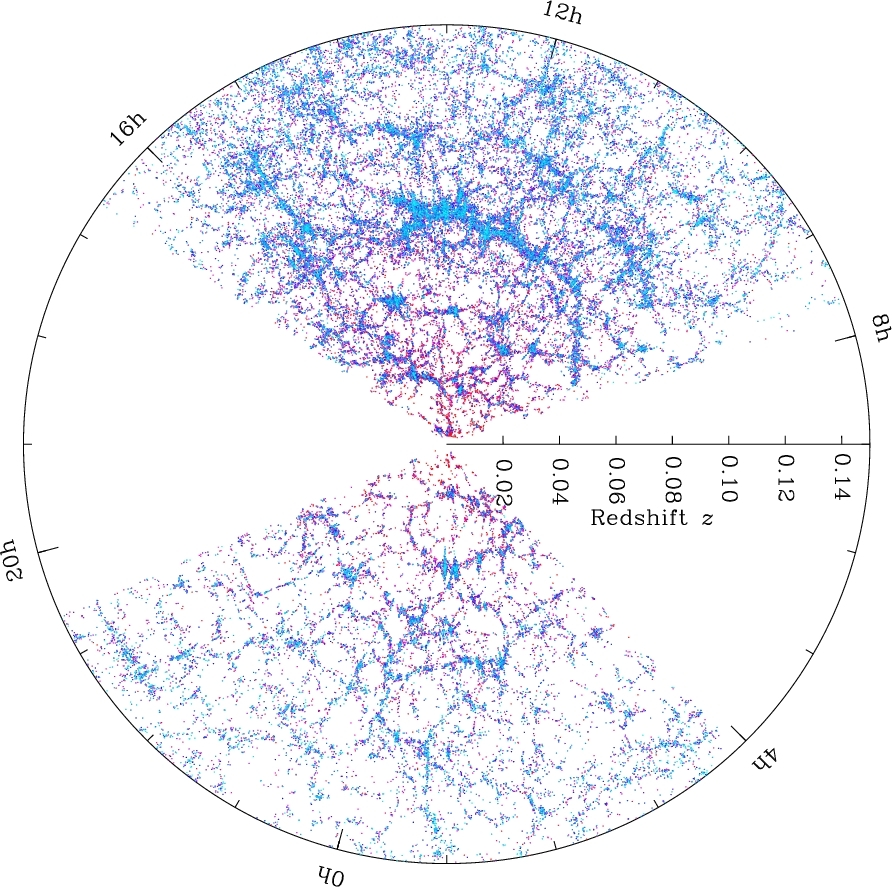
\includegraphics[width=0.9\columnwidth]{images/misc/orangepie.jpg}%
    
    \caption{
    Galaxy map from the Sloan Digital Sky Survey.
    }
    
    \label{fig:1.2}
\end{figure}


\section{The Missing Link (Reconstruction)}

\todo[inline]{Motivate our desire to link the two and talk about the problems we have (Dark Ages)}

\todo[inline]{Motivate the desire to reconstruct the BAO feature}
